The goal of this project is to parallelize a serial code, inspired in a
radiative transfer code.

The serial code is given below. As you can see, the only input to the program
are the number of points in the X and Y dimensions (\textit{nx, ny}) used to
allocate array with the given sizes. This is initialized (\textit{init\_atmos()})
with some arbitrary data, and then the code calls \textit{rt\_l}), which performs
what you can graphically see in figure \ref{fig:rt-ser}: we simulate 45º rays in
a non-periodic domain, so we \textit{follow} the rays starting in the first
column and in the last row throughout the domain, applying a simple expression
(see procedure \textit{propagate()}) to recalculate the values in the
array. Lastly, with the proocedure \textit{print\_atmos()} we can compare the
initial with the final values.

\begin{verbatim}

PROGRAM RT_LIKE
  IMPLICIT NONE

  DOUBLE PRECISION, DIMENSION(:,:), ALLOCATABLE :: atmos
  INTEGER :: nx,ny
  
  READ*, nx,ny
  ALLOCATE(atmos(nx,ny))

  !! Initialize array with some sample data
  CALL init_atmos()

  PRINT*, " ------------ Initial values -----------------"
  CALL print_atmos()

  PRINT*, ""
  CALL rt_l()
  PRINT*, ""
  
  PRINT*, " ------------ Final values -----------------"
  CALL print_atmos()
  
CONTAINS

  ! --------------------------------------------
  ! rt_l
  !
  ! This routine is fixed for 45º angles
  ! --------------------------------------------
  SUBROUTINE rt_l()
    INTEGER :: st_row,st_col,uw_row,uw_col,dw_row,dw_col

    ! Rays starting in column 1
    DO st_row=1,nx
       uw_row = st_row
       uw_col = 1
!       PRINT*, "Doing ray starting at:", uw_row,uw_col
       CALL propagate(uw_row,uw_col)
    END DO

    ! Rays starting in row nx
    DO st_col=2,ny
       uw_row = nx
       uw_col = st_col
!       PRINT*, "Doing ray starting at;", uw_row,uw_col
       CALL propagate(uw_row,uw_col)
    END DO
  END SUBROUTINE rt_l
  
  ! --------------------------------------------
  ! propagate
  !
  ! --------------------------------------------
  SUBROUTINE propagate(uw_row,uw_col)
    INTEGER :: uw_row,uw_col,dw_row,dw_col

    DO
       dw_row = uw_row - 1
       dw_col = uw_col + 1
       IF (dw_row < 1 .OR. dw_col > ny) EXIT
       atmos(dw_row,dw_col) = (atmos(uw_row,uw_col) + atmos(dw_row,dw_col)) * 0.5
!       PRINT*, "pos",dw_row,dw_col,atmos(uw_row,uw_col),atmos(dw_row,dw_col)
       uw_row = dw_row
       uw_col = dw_col
    END DO
  END SUBROUTINE propagate

  ! --------------------------------------------
  ! init_atmos
  !
  ! --------------------------------------------
  SUBROUTINE init_atmos()
    INTEGER :: x,y
    
    DO x=1,nx
       DO y=1,ny
          atmos(x,y) = 1.234 * x + 2.345 * y
       END DO
    END DO
  END SUBROUTINE init_atmos

  ! --------------------------------------------
  ! print_atmos
  !
  ! --------------------------------------------
  SUBROUTINE print_atmos()
    INTEGER :: x
    CHARACTER(LEN=50) :: fmt

    write(fmt,*) "(" , ny , "E10.3)"
    DO x=1,nx
       WRITE(*,fmt) atmos(x,:)
    END DO
  END SUBROUTINE print_atmos
  
END PROGRAM RT_LIKE
\end{verbatim}

\begin{figure}[!htbp]
  \centering
  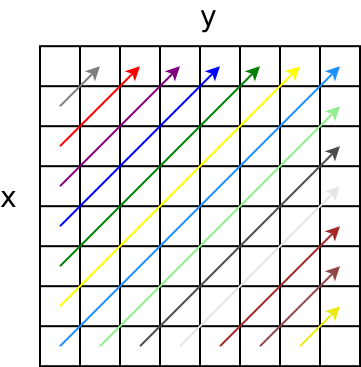
\includegraphics[width=0.4\textwidth]{graphics/projects/rt-ser.png}
  \label{fig:rt-ser}
  \caption{RT serial}
\end{figure}

We can see that the serial code can work for any array size. For example, below
we show runs for array sizes 4x4 and 7x9

\begin{verbatim}


[angelv]$ ./rt-serial
4 4
  ------------ Initial values -----------------
 0.358E+01 0.592E+01 0.827E+01 0.106E+02
 0.481E+01 0.716E+01 0.950E+01 0.118E+02
 0.605E+01 0.839E+01 0.107E+02 0.131E+02
 0.728E+01 0.963E+01 0.120E+02 0.143E+02
 
 
  ------------ Final values -----------------
 0.358E+01 0.537E+01 0.744E+01 0.964E+01
 0.481E+01 0.660E+01 0.867E+01 0.110E+02
 0.605E+01 0.784E+01 0.102E+02 0.125E+02
 0.728E+01 0.963E+01 0.120E+02 0.143E+02



[angelv]$ ./rt-serial
7 9
  ------------ Initial values -----------------
 0.358E+01 0.592E+01 0.827E+01 0.106E+02 0.130E+02 0.153E+02 0.176E+02 0.200E+02 0.223E+02
 0.481E+01 0.716E+01 0.950E+01 0.118E+02 0.142E+02 0.165E+02 0.189E+02 0.212E+02 0.236E+02
 0.605E+01 0.839E+01 0.107E+02 0.131E+02 0.154E+02 0.178E+02 0.201E+02 0.225E+02 0.248E+02
 0.728E+01 0.963E+01 0.120E+02 0.143E+02 0.167E+02 0.190E+02 0.214E+02 0.237E+02 0.260E+02
 0.852E+01 0.109E+02 0.132E+02 0.156E+02 0.179E+02 0.202E+02 0.226E+02 0.249E+02 0.273E+02
 0.975E+01 0.121E+02 0.144E+02 0.168E+02 0.191E+02 0.215E+02 0.238E+02 0.262E+02 0.285E+02
 0.110E+02 0.133E+02 0.157E+02 0.180E+02 0.204E+02 0.227E+02 0.251E+02 0.274E+02 0.297E+02
 
 
  ------------ Final values -----------------
 0.358E+01 0.537E+01 0.744E+01 0.964E+01 0.119E+02 0.142E+02 0.166E+02 0.189E+02 0.212E+02
 0.481E+01 0.660E+01 0.867E+01 0.109E+02 0.132E+02 0.155E+02 0.178E+02 0.202E+02 0.225E+02
 0.605E+01 0.784E+01 0.990E+01 0.121E+02 0.144E+02 0.167E+02 0.191E+02 0.214E+02 0.238E+02
 0.728E+01 0.907E+01 0.111E+02 0.133E+02 0.157E+02 0.180E+02 0.204E+02 0.227E+02 0.251E+02
 0.852E+01 0.103E+02 0.124E+02 0.147E+02 0.171E+02 0.194E+02 0.218E+02 0.241E+02 0.264E+02
 0.975E+01 0.115E+02 0.139E+02 0.162E+02 0.186E+02 0.209E+02 0.233E+02 0.256E+02 0.280E+02
 0.110E+02 0.133E+02 0.157E+02 0.180E+02 0.204E+02 0.227E+02 0.251E+02 0.274E+02 0.297E+02
\end{verbatim}


Your goal then is to parallelize this code. You can assume that rank 0
initializes the whole array (which is useful for printing), and then it is
scattered amongst all the processes, which will run the procedure
\textit{rt\_l()} on their local chunk of the array, then gathered again in
rank 0 to print the final value. In the parallel code, besides getting the size
of the array (\textit{nx, ny}), you should also get as input the number of
blocks you will do in every dimension \textit{blocks\_x, blockx\_y}, so that the
number of total processes in your parallel run is \textit{blocks\_x *
  blocks\_y}. To clarify with one example, see figure \ref{fig:rt-par}. There,
nx=8 and ny=8, and we want to use 4 processes (i.e., we will run the code as
\textit{mpirun -np 4 [...]}). The number of blocks in X is 2, and the number of
blocks in Y is also 2, so each process will end up working with a chunk of
size=4x4 (but will need to make the local array bigger with ghost cells in order
to store the corresponding values from the neighbour processes).


\begin{figure}[!htbp]
  \centering
  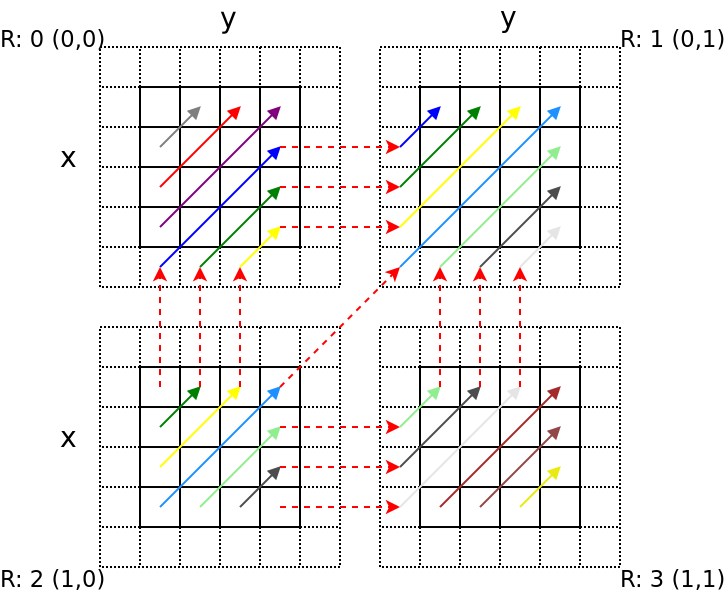
\includegraphics[width=0.6\textwidth]{graphics/projects/rt-par.png}
  \label{fig:rt-par}
  \caption{RT parallel}
\end{figure}

The idea here is quite similar to the heat2D exercise in
\ref{ex:collective-mpi-heat2d}, so you can reuse some of the code from the
solution to that exercise. When making the code generic, you will probably find
useful to create a cartesian distribution of processes, so for example the
process 0 in figure \ref{fig:rt-par} (with label ``R: 0 (0,0)'') could have
process coordinates (0,0) while process with rank 3 (``R: 3 (1,1)'') would have
process coordinates (1,1). Knowing which process row and/or column a process is
in, will be crucial to understand in which order it has to perform the
receive/send operations, where to start propagating the rays, etc.

The idea is not too difficult, but it can get confusing with indexes,
etc. quickly, so start assuming that you will always run it with 4 processes in
a distribution as per figure \ref{fig:rt-par} and with a number of grid cells
that is divisible by 2. This will give you an idea of the difficulties with
indexes, etc. but it should be relatively easy. \textbf{If your code works up to
  here, getting \textit{EXACTLY} the same final values as in the serial version,
  you would get 7 out of 10 points for this project}.

The next step would be to make the work code with other processes numbers and
distributions, but still assuming that the number of cells in each dimension is
divisible by the number of blocks in that dimension, so all processes end up
with chunks of the same size. \textbf{If you are able to get it to work up to here,
then you will have full marks for this project.}

\textbf{EXTRA POINTS: If you are able to make it work for any distribution but
  also for a number of cells not divisible by the number of blocks, then this
  will give you full marks in this project, but also 1 point more in the final
  mark of the course (10 being the maximum possible mark).}

Below you can see executions of my solution for the array sizes as per the
serial code above. The first one (4x4 and 2 blocks in each dimension should be
your first goal, where each process will have a chunk of 2x2).

\begin{verbatim}


[angelv]$ mpirun -np 4 rt-par 
 Global array dimensions?
4 4
 Number of blocks (x,y)?
2 2
  ------------ Initial values -----------------
 0.358E+01 0.592E+01 0.827E+01 0.106E+02
 0.481E+01 0.716E+01 0.950E+01 0.118E+02
 0.605E+01 0.839E+01 0.107E+02 0.131E+02
 0.728E+01 0.963E+01 0.120E+02 0.143E+02
 
 
  ------------ Final values -----------------
 0.358E+01 0.537E+01 0.744E+01 0.964E+01
 0.481E+01 0.660E+01 0.867E+01 0.110E+02
 0.605E+01 0.784E+01 0.102E+02 0.125E+02
 0.728E+01 0.963E+01 0.120E+02 0.143E+02



[angelv]$ mpirun --oversubscribe -np 12 rt-par 
 Global array dimensions?
7 9
 Number of blocks (x,y)?
3 4
  ------------ Initial values -----------------
 0.358E+01 0.592E+01 0.827E+01 0.106E+02 0.130E+02 0.153E+02 0.176E+02 0.200E+02 0.223E+02
 0.481E+01 0.716E+01 0.950E+01 0.118E+02 0.142E+02 0.165E+02 0.189E+02 0.212E+02 0.236E+02
 0.605E+01 0.839E+01 0.107E+02 0.131E+02 0.154E+02 0.178E+02 0.201E+02 0.225E+02 0.248E+02
 0.728E+01 0.963E+01 0.120E+02 0.143E+02 0.167E+02 0.190E+02 0.214E+02 0.237E+02 0.260E+02
 0.852E+01 0.109E+02 0.132E+02 0.156E+02 0.179E+02 0.202E+02 0.226E+02 0.249E+02 0.273E+02
 0.975E+01 0.121E+02 0.144E+02 0.168E+02 0.191E+02 0.215E+02 0.238E+02 0.262E+02 0.285E+02
 0.110E+02 0.133E+02 0.157E+02 0.180E+02 0.204E+02 0.227E+02 0.251E+02 0.274E+02 0.297E+02
 
 
  ------------ Final values -----------------
 0.358E+01 0.537E+01 0.744E+01 0.964E+01 0.119E+02 0.142E+02 0.166E+02 0.189E+02 0.212E+02
 0.481E+01 0.660E+01 0.867E+01 0.109E+02 0.132E+02 0.155E+02 0.178E+02 0.202E+02 0.225E+02
 0.605E+01 0.784E+01 0.990E+01 0.121E+02 0.144E+02 0.167E+02 0.191E+02 0.214E+02 0.238E+02
 0.728E+01 0.907E+01 0.111E+02 0.133E+02 0.157E+02 0.180E+02 0.204E+02 0.227E+02 0.251E+02
 0.852E+01 0.103E+02 0.124E+02 0.147E+02 0.171E+02 0.194E+02 0.218E+02 0.241E+02 0.264E+02
 0.975E+01 0.115E+02 0.139E+02 0.162E+02 0.186E+02 0.209E+02 0.233E+02 0.256E+02 0.280E+02
 0.110E+02 0.133E+02 0.157E+02 0.180E+02 0.204E+02 0.227E+02 0.251E+02 0.274E+02 0.297E+02
\end{verbatim}

The second one is the most generic one (and probably quite difficult to get
right). The number of cells in x is 7 and we want to divide them in 3 blocks, so
two blocks should have two cells in x while another one should have 3 cells,
etc.  In case it is not clear, the way my code distributes the 12 processes in
chunks is as follows:

\begin{verbatim}
| 3x3 | 3x2 | 3x2 | 3x2 |
| 2x3 | 2x2 | 2x2 | 2x2 |
| 2x3 | 2x2 | 2x2 | 2x2 |
\end{verbatim}

This is not easy, but it is not too difficult either. Start with the 4 process
division, which will help you to understand which things have to be generalized
in order to be able to get it to work with an arbitrary distribution.

